\newpage


\lstset{
  escapeinside={(*}{*)},
}
\section{Problem 5 (15 pts)}
\begin{enumerate}
    \item Define operations \textit{Enqueue}($\mathscr{Q}, \mathscr{T}$) and \textit{Dequeue}($\mathscr{Q}$).\\
    \begin{itemize}
        \item \textit{Enqueue}($\mathscr{Q}, \mathscr{T}$) is an operation that is used to insert an element to the rear end of the queue. In this case, the queue ADT is defined using two stack $\Sigma_{1}$ and $\Sigma_{2}$. In order to implement the enqueue operation, it can use the push() operation of the Stack ADT to complete. In addition, the Stack ADT is implemented using List $\Lambda$, so the push() operation could be implemented using the cons() operation of the List $\Lambda$, it adds an element at the top of the Stack. Therefore, using cons() operation of the List to implement push() operation of Stack, and then implement Enqueue() operation of Queue ADT. This allows to insert an element at the rear end of the queue (enqueue).\\ \\
        \begin{lstlisting}
            push((*$\Lambda$*), T) is
                cons(T, (*$\Lambda$*))
                
            enqueue(Q, T) is
                push(Q, T)
        \end{lstlisting}
        
        \item \textit{Dequeue}($\mathscr{Q}$) is an operation of Queue ADT that removes an element from the front end of the queue. Because the Queue ADT is implemented using two Stacks $\Sigma_{1}$ and $\Sigma_{2}$, the elements will be moved from a stack to another stack, e.g from $\Sigma_{1}$ to $\Sigma_{2}$, by using push() operation to gradually add to the top of $\Sigma_{2}$ the element of the top of $\Sigma_{1}$. Eventually, the top of $\Sigma_{2}$ is the front end of the Queue ADT. Then this front end can be removed using pop() operation of Stack, in which this pop() operation is implemented using head() and tail() operations (car, cdr).\\ \\
        \begin{lstlisting}[mathscape]
            pop(stack) is
                if not(isEmpty((*$\Lambda$*)))
                    el = g()
                    (*$\Lambda$*)' = f((*$\Lambda$*))
                return el

            dequeue(Q)
                if (isEmpty((*$\Sigma_{1}$*)) && isEmpty((*$\Sigma_{2}$*)) )
                    nil
                if (isEmpty((*$\Sigma_{2}$*)))
                    while(not(isEmpty((*$\Sigma_{1}$*))))
                        push((*$\Sigma_{2}$*), pop((*$\Sigma_{1}$*)))
                return pop(((*$\Sigma_{2}$*)))
        \end{lstlisting}
    \end{itemize}



    \item Use Common LISP to define two stacks (\texttt{stack1} and
\texttt{stack2}) as global variables to hold the collection, and implement functions \texttt{enqueue}
and \texttt{dequeue}. Place your code in file \texttt{queue-adt.lisp}, and include your interaction
with the language environment to demonstrate the behavior of your code.\\ \\
The Code for the implementations of Enqueue and Dequeue: 
\begin{lstlisting}
(defun push (stack element)
  (cons element stack))

(defun pop (stack)
  (if (null stack)
      (error "Stack is empty")
      (values (car stack) (cdr stack))))

(defun stack-empty? (stack)
  (null stack))

(defun enqueue (queue element)
  (setf (symbol-value 's1) (push (symbol-value 's1) element)))

(defun dequeue (queue)
  (if (stack-empty? (symbol-value 's2))
      (progn
        (while (not (stack-empty? (symbol-value 's1)))
          (multiple-value-bind (element remaining-stack) 
          (pop (symbol-value 's1))
            (setf (symbol-value 's2) 
            (push (symbol-value 's2) element))))
        (if (stack-empty? (symbol-value 's2))
            (error "Queue is empty")))
      nil)
  (multiple-value-bind (element remaining-stack) 
  (pop (symbol-value 's2))
    (setf (symbol-value 's2) remaining-stack)
    element))
\end{lstlisting}
\newpage
The interation with Queue ADT: \\ \\ 

(setq s1 nil) ;Initialize $\Sigma_1$ stack \\
(setq s2 nil) ;Initialize $\Sigma_2$ Stack \\

(enqueue 'q 'a)\\
(enqueue 'q 'b)\\
(enqueue 'q 'c)\\\\
(print (dequeue 'q))\\
$\mathbb{>}$A\\
(print (dequeue 'q))\\
$\mathbb{>}$B\\
(print (dequeue 'q))\\
$\mathbb{>}$C\\

    \item Implement operations \textit{head}, \textit{tail} and \textit{cons} in Prolog and demonstrate their usage (include your interaction with the language environment in your submission).
\\
    \begin{figure}[hbt!]
        \centering
        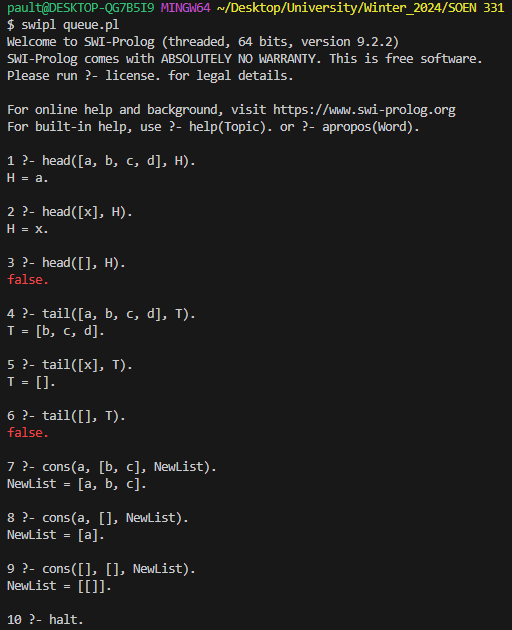
\includegraphics[scale=0.6]{assigment1/331A1_num5_part3.png}
        \caption{Prolog interaction for problem 5 part 3}
    \end{figure}
    
\end{enumerate}